\documentclass[8pt,aspectratio=169]{beamer}
\usetheme{metropolis} 
\usepackage[utf8]{inputenc}
\usepackage[T1]{fontenc}
\usepackage[english]{babel}
\usepackage{amsmath}
\usepackage{amsfonts}
\usepackage{amssymb}
\usepackage{graphicx}
\usepackage{tikz}
\usetikzlibrary{positioning, shapes.geometric, trees}
\usetheme{default}
\usepackage{listings}
\usepackage{fontawesome5}




\begin{document}
	\author{Pierre Schaus \& Guillaume Derval}
	\title{A quick summary of the LINFO1121 course material}
	%\subtitle{}
	%\logo{}
	%\institute{}
	%\date{}
	%\subject{}
	%\setbeamercovered{transparent}
	%\setbeamertemplate{navigation symbols}{}

	\begin{frame}[plain]
	\maketitle
	\end{frame}

\begin{frame}[t]
\frametitle{Disclaimer \& Learning Resources}

\begin{alertblock}{Warning: Not Self-Contained}
These slides are a \textbf{summary and mnemonic aid} only. They do not contain the full course material required for the exam.
\end{alertblock}

\vspace{0.3cm}
\textbf{Official Course Content:}
\begin{itemize}
    \item \textbf{Theory:} The official website (slides, chapters to read, theoretical exercises and links to inginious exercises)\\ 
    \small \url{https://pschaus.github.io/LINFO1121/}
    \item \textbf{Practice:} All \textbf{INGInious} exercises:\\
    \small \url{https://inginious.info.ucl.ac.be/course/LINFO1121}
    \item \textbf{Reference:} Related chapters of \textit{Algorithms, 4th Edition} by \textbf{Sedgewick \& Wayne}.
\end{itemize}

\vspace{0.4cm}
\begin{center}
    \color{red} \textbf{Course Material = Website + INGInious + Book Chapters}
\end{center}

\vspace{0.2cm}
\footnotesize \textit{Contributions are welcome! Submit a Pull Request at:} \\
\url{https://github.com/pschaus/LINFO1121-summary}

\end{frame}


\begin{frame}[t, fragile]
\frametitle{The Iterable and Iterator Pattern}

\begin{columns}[T]
    % Left Column: Theory
    \begin{column}{0.45\textwidth}
        \textbf{The Interfaces}
        \begin{itemize}
            \item \textbf{Iterable<T>}: A collection that can be the target of a "for-each" loop. Requires method \texttt{iterator()}.
            \item \textbf{Iterator<T>}: The object that tracks the state of the traversal.
            \item \textbf{Why Inner Classes?} The iterator needs access to the private array/data of the container.
        \end{itemize}
    \end{column}

    % Right Column: Code
    \begin{column}{0.55\textwidth}
\begin{lstlisting}[language=Java, basicstyle=\tiny\ttfamily, keywordstyle=\color{blue}, frame=single]
public class MyList<T> implements Iterable<T> {
    private T[] items;
    private int size;

    @Override
    public Iterator<T> iterator() {
        return new ListIterator();
    }

    private class ListIterator implements Iterator<T> {
        private int cursor = 0;
        
        public boolean hasNext() {
            return cursor < size;
        }
        
        public T next() {
            if (!hasNext()) throw new NoSuchElementException();
            return items[cursor++];
        }
    }
}
\end{lstlisting}
    \end{column}
\end{columns}
\end{frame}


\begin{frame}[t, fragile]
\frametitle{Iteration Strategies: Fail-Fast vs. Fail-Safe}

\begin{columns}[T]
    % Left Column: Strategy Explanation
    \begin{column}{0.48\textwidth}
        \textbf{The Problem:} Structural changes (add/remove) during iteration can lead to undefined behavior.
        
        \vspace{0.2cm}
        \textbf{1. Fail-Fast (frequent in Java collections)}
        \begin{itemize}
            \item Throws \texttt{ConcurrentModificationException} immediately if the collection changes.
            \item \textbf{Pros:} Detects bugs early; no memory overhead.
            \item \textbf{Cons:} Unsuitable for highly concurrent environments.
        \end{itemize}

        \textbf{2. Fail-Safe}
        \begin{itemize}
            \item Works on a \textbf{snapshot/copy} of the data.
            \item \textbf{Pros:} No exception thrown; thread-safe.
            \item \textbf{Cons:} Overhead of copying; might not see recent updates.
        \end{itemize}
    \end{column}

    % Right Column: The Implementation
    \begin{column}{0.52\textwidth}

\begin{lstlisting}[language=Java, basicstyle=\tiny\ttfamily, keywordstyle=\color{blue}, frame=single]
public class MyList<E> {
    // Structural version of the list
    protected int modCount = 0; 

    public Iterator<E> iterator() {
        return new Itr(); // Snapshot taken here!
    }

    private class Itr implements Iterator<E> {
        // Snapshot of modCount at creation
        int expectedModCount = modCount;

        public E next() {
            checkForComodification();
            // ... return next element
        }

        final void checkForComodification() {
            // Compare current state vs creation state
            if (modCount != expectedModCount)
                throw new ConcurrentModificationException();
        }
    }
}
\end{lstlisting}
    \end{column}
\end{columns}
\end{frame}



% \section{Existing implementations of ADTs in Java}

\begin{frame}{Existing implementations of ADTs in Java}
These slides spend a few minutes on the implementations of the different ADTs seen in the course. They mix "pure" ADTs (without implementation) with ADTs "pre-implemented" by Java.
It's up to you to know the difference between an ADT and an implementation ;-)

When you see a complexity in red, and you plan to use this method in a data structure, it probably means that you have chosen the wrong data structure.

All methods that are not listed are generally non-standard AND expensive, so they should be avoided. The Javadoc is your friend.

You are not safe from an error in these slides ;-)
\end{frame}

\begin{frame}
\frametitle{Arrays (non-dynamic)}
\centering
\begin{tabular}{lll}
	Usefulness & \multicolumn{2}{l}{Storage of a known number of elements}\\
	Constraint & \multicolumn{2}{l}{Fixed number of elements}\\
	Instantiation & \multicolumn{2}{l}{\texttt{new Type[size]} (e.g.: \texttt{new int[8]})}\\
\end{tabular}\\
\vspace{0.5cm}
\centering
\begin{tabular}{lll}
	\multicolumn{3}{c}{\textbf{Methods}} \\
	\textit{Name} & \textit{Java} & \textit{Complexity} \\
	Access element \texttt{i} & \texttt{array[i]} & $\Theta(1)$\\
	Assign \texttt{x} to element \texttt{i} & \texttt{array[i] = x} & $\Theta(1)$\\
\end{tabular}
\end{frame}

\begin{frame}
\frametitle{Arrays (dynamic)}
\centering
\begin{tabular}{ll}
	Usefulness & Storage of elements, random access\\
	Instantiation & \texttt{new ArrayList<Type>()}\\
\end{tabular}\\
\vspace{0.5cm}
\centering
\begin{tabular}{lll}
	\multicolumn{3}{c}{\textbf{Methods} on an object \texttt{o} of size $n$} \\
	\textit{Name} & \textit{Java} & \textit{Complexity} \\
	Access element \texttt{i} & \texttt{o.get(i)} & $\Theta(1)$\\
	Assign \texttt{x} to element \texttt{i} & \texttt{o.set(i, x)} & $\Theta(1)$\\
	Add at the end & \texttt{o.add(x)} & $\Theta(1)$ \color{orange}amortized\\
	Remove from the end & \texttt{o.remove(n-1)} & $\Theta(1)$ \color{orange}amortized\\
	Add anywhere & \texttt{o.add(i, x)} & $\color{red}\mathcal{O}(n)$\\
	Remove from anywhere & \texttt{o.remove(i)} & $\color{red}\mathcal{O}(n)$\\
	Contains \texttt{x}? & \texttt{o.contains(x)} & $\color{red}\mathcal{O}(n)$\\
\end{tabular}
\end{frame}

\begin{frame}
\frametitle{Doubly linked lists}
\centering
\begin{tabular}{ll}
	Usefulness & Storage of elements, sequential access\\
	Instantiation & \texttt{new LinkedList<Type>()}\\
\end{tabular}\\
\vspace{0.5cm}
\centering
\begin{tabular}{lll}
	\multicolumn{3}{c}{\textbf{Methods} on an object \texttt{o} of size $n$} \\
	\textit{Name} & \textit{Java} & \textit{Complexity} \\
	Access first element & \texttt{o.getFirst()} & $\Theta(1)$\\
	Add to front & \texttt{o.addFirst(x)} & $\Theta(1)$\\
	Remove from front & \texttt{o.removeFirst()} & $\Theta(1)$\\
	Access last element & \texttt{o.getLast()} & $\Theta(1)$\\
	Add to back & \texttt{o.addLast(x)} & $\Theta(1)$\\
	Remove from back & \texttt{o.removeLast()} & $\Theta(1)$\\
	Access element \texttt{i} & \texttt{o.get(i)} & $\color{red}\mathcal{O}(n)$\\
	Assign \texttt{x} to element \texttt{i} & \texttt{o.set(i, x)} & $\color{red}\mathcal{O}(n)$\\
	Add anywhere & \texttt{o.add(i, x)} & $\color{red}\mathcal{O}(n)$\\
	Remove from anywhere & \texttt{o.remove(i)} & $\color{red}\mathcal{O}(n)$\\
	Contains \texttt{x}? & \texttt{o.contains(x)} & $\color{red}\mathcal{O}(n)$\\
\end{tabular}
\end{frame}

\begin{frame}
\frametitle{Queue}
\centering
\begin{tabular}{ll}
	Usefulness & First-in, first-out (FIFO)\\
	Instantiation & \texttt{Queue<Type> o = new LinkedList<>()}\\
	& \color{red} (\texttt{Queue} is an interface in Java!)\\
\end{tabular}\\
\vspace{0.5cm}
\centering
\begin{tabular}{lll}
	\multicolumn{3}{c}{\textbf{Methods} on an object \texttt{o} of size $n$} \\
	\textit{Name} & \textit{Java} & \textit{Complexity} \\
	Access first element & \texttt{o.element()} & $\Theta(1)$\\
	Add (at the end) & \texttt{o.add(x)} & $\Theta(1)$\\
	Remove (from the front) & \texttt{o.remove()} & $\Theta(1)$\\
\end{tabular}\\
\vspace{0.5cm}
\color{blue} When using the Queue ADT, you should NEVER have to use other methods (except \texttt{size} and \texttt{empty}).

\color{blue} Be careful, these functions can throw exceptions if the Queue is empty.
\end{frame}

\begin{frame}
\frametitle{Stack}
\centering
\begin{tabular}{ll}
	Usefulness & Last-in, first-out (LIFO)\\
	Instantiation & \texttt{Stack<Type> o = new Stack<>()}
\end{tabular}\\
\vspace{0.5cm}
\centering
\begin{tabular}{lll}
	\multicolumn{3}{c}{\textbf{Methods} on an object \texttt{o} of size $n$} \\
	\textit{Name} & \textit{Java} & \textit{Complexity} \\
	Access the element on top of the stack & \texttt{o.peek()} & $\Theta(1)$\\
	Add (on top) & \texttt{o.push(x)} & $\Theta(1)$\\
	Remove (from top) & \texttt{o.pop()} & $\Theta(1)$\\
\end{tabular}\\
\vspace{0.5cm}
\color{blue} When using the Stack ADT, you should NEVER have to use other methods (except \texttt{size} and \texttt{empty}).

\color{blue} You can (but are not \textit{required} to) also take a look at the Deque interface (double-ended queue, which implements both the Stack and Queue ADTs) and its implementations: \texttt{LinkedList} and \texttt{ArrayDeque}.

\color{red} NEVER iterate (foreach or \texttt{iterator}) over a stack. The elements are returned in reverse order...

\end{frame}

\begin{frame}
\frametitle{Sorted list (custom)}
\centering
\begin{tabular}{ll}
	Usefulness & Storage of elements in a sorted manner\\
	Instantiation & To be implemented by yourself from LinkedList\\
	& \color{red} In practice, I don't see when this could be useful. \\
	& \color{red} Only here to be able to compare with what follows.
	
\end{tabular}\\
\vspace{0.5cm}
\centering
\begin{tabular}{ll}
	\multicolumn{2}{c}{\textbf{Methods} on an object \texttt{o} of size $n$} \\
	\textit{Name} & \textit{Complexity} \\
	Add to the right place & $\color{red}\mathcal{O}(n)$\\
    Remove smallest/largest & $\Theta(1)$\\
    Contains? & $\color{red}\mathcal{O}(n)$\\
\end{tabular}\\
\vspace{0.5cm}
\end{frame}

\begin{frame}
\frametitle{Sorted array (custom)}
\centering
\begin{tabular}{ll}
	Usefulness & Storage of elements in a sorted manner\\
	Instantiation & To be implemented by yourself from an ArrayList or a Java array\\
	& \color{red} In practice, I don't see when this could be useful. \\
	& \color{red} Only here to be able to compare with what follows.
	
\end{tabular}\\
\vspace{0.5cm}
\centering
\begin{tabular}{ll}
	\multicolumn{2}{c}{\textbf{Methods} on an object \texttt{o} of size $n$} \\
	\textit{Name} & \textit{Complexity} \\
	Add to the right place & $\color{red}\mathcal{O}(n)$\\
	Remove the smallest & $\color{red}\Theta(n)$\\
	Remove the largest & $\Theta(1)$\\
	Contains? & $\mathcal{O}(\log n)$ (binary search)\\
\end{tabular}\\
\vspace{0.5cm}
\end{frame}


\begin{frame}[t, fragile]
\frametitle{Sorting in Java: Arrays and Collections}

\begin{columns}[T]
    % --- Left Column: Basics ---
    \begin{column}{0.48\textwidth}
        \textbf{1. Primitive Arrays}
        \begin{itemize}
            \item Use \texttt{Arrays.sort(arr)}.
            \item Implementation of a variant of quicksort in $O(N \log N)$.
        \end{itemize}

        \vspace{0.2cm}
        \textbf{2. Objects \& Collections}
        \begin{itemize}
            \item Use \texttt{list.sort()} or \texttt{Collections.sort(list)}. It requires objects to implement \texttt{Comparable} (defines "natural order").
            \item You can also pass a custom comparator in argument (more flexible).
            \item Implementation of variant of quicksort in $O(N \log N)$ (stable).
        \end{itemize}
    \end{column}

    % --- Right Column: Custom Sorting ---
    \begin{column}{0.52\textwidth}
        \textbf{3. Custom Order (Comparators)}
        \textit{Using Lambda expressions:}
\begin{lstlisting}[language=Java, basicstyle=\tiny\ttfamily, frame=single]
// Standard Lambda notation
list.sort((a, b) -> a.val - b.val);

// Using Comparator factory methods
list.sort(Comparator.comparing(Node::getVal));

// Lexico-graphic: criterion one, then second in case of ties
list.sort(Comparator.comparing(Node::getCategory)
                    .thenComparing(Node::getVal));
\end{lstlisting}
    \end{column}
\end{columns}
\end{frame}

\begin{frame}
\frametitle{TreeSet: Self-balancing tree (set)}
\centering
\begin{tabular}{ll}
	Usefulness & Set, sorted\\
	Instantiation & \texttt{new TreeSet<Type>}\\
	What is it? & Behind the scenes, it's a red-black tree\\
	& \color{red} No duplicates (it's a set)\\
	& \color{red} Elements must be comparable
	
\end{tabular}\\
\centering
\begin{tabular}{lll}
	\multicolumn{3}{c}{\textbf{Methods} on an object \texttt{o} of size $n$} \\
	\textit{Name} & \textit{Java} & \textit{Complexity} \\
	Add & \texttt{o.add(x)} & $\mathcal{O}(\log n)$\\
	Remove & \texttt{o.remove(x)} & $\mathcal{O}(\log n)$\\
	Contains? & \texttt{o.contains(x)} & $\mathcal{O}(\log n)$\\
	Find element below (or =) & \texttt{o.floor(x)} & $\mathcal{O}(\log n)$\\
	Find element above (or =) & \texttt{o.ceil(x)} & $\mathcal{O}(\log n)$\\
	Find element strictly below & \texttt{o.higher(x)} & $\mathcal{O}(\log n)$\\
	Find element strictly above & \texttt{o.lower(x)} & $\mathcal{O}(\log n)$\\
\end{tabular}\\
\vspace{0.5cm}
\color{blue} Another useful method: \texttt{subset}, which allows extracting a part of the tree at constant cost. \texttt{descendingIterator} is also very practical.
\end{frame}

\begin{frame}
\frametitle{HashSet: hash table (set)}
\centering
\begin{tabular}{ll}
	Usefulness & Set\\
	Instantiation & \texttt{new HashSet<Type>}\\
	What is it? & A hash table\\
	& \color{red} No duplicates (it's a set)\\
	& \color{red} Elements must be hashable (!!!)\\
	& \color{red} Unsorted
	
\end{tabular}\\
\vspace{0.5cm}
\centering
\begin{tabular}{lll}
	\multicolumn{3}{c}{\textbf{Methods} on an object \texttt{o} of size $n$} \\
	\textit{Name} & \textit{Java} & \textit{Complexity} \\
	Add & \texttt{o.add(x)} & $\mathcal{O}(1)$ \color{orange} amortized\\
	Remove & \texttt{o.remove(x)} & $\mathcal{O}(1)$ \color{orange} amortized\\
	Contains? & \texttt{o.contains(x)} & $\mathcal{O}(1)$ \color{orange} amortized\\
\end{tabular}\\
\vspace{0.5cm}
\color{blue} Under the constraint that the hashes are well distributed!
\end{frame}

\begin{frame}
\frametitle{TreeMap: self-balancing tree (dictionary)}
\centering
\begin{tabular}{ll}
	Usefulness & Dictionary\\
	Instantiation & \texttt{new TreeMap<TypeKey,TypeValue>}\\
	What is it? & A red-black tree (or equivalent)\\
	& \color{red} No duplicate keys (it's a dictionary)\\
	& \color{red} Keys must be comparable
\end{tabular}\\
\vspace{0.5cm}
\centering
\begin{tabular}{lll}
	\multicolumn{3}{c}{\textbf{Methods} on an object \texttt{o} of size $n$} \\
	\textit{Name} & \textit{Java} & \textit{Complexity} \\
	Add (key \texttt{x}, value \texttt{y})& \texttt{o.put(x, y)} & $\mathcal{O}(\log n)$\\
	Get key & \texttt{o.get(x)} & $\mathcal{O}(\log n)$\\
	Remove key & \texttt{o.remove(x)} & $\mathcal{O}(\log n)$\\
	Contains key? & \texttt{o.containsKey(x)} & $\mathcal{O}(\log n)$\\
\end{tabular}\\
\vspace{0.5cm}
\color{blue} TreeSet functions are also available for keys (\texttt{ceilingKey}, \texttt{subMap}...).

\color{blue} See later slide for a tip on iterating over Maps and especially TreeMaps.

\color{red} Even if there are methods to search for values (\texttt{containsValue}, ...), they are generally in $\mathcal{O}(n)$.
\end{frame}

\begin{frame}
\frametitle{HashMap: hash table (dictionary)}
\centering
\begin{tabular}{ll}
	Usefulness & Set\\
	Instantiation & \texttt{new HashMap<TypeKey,TypeValue>}\\
	What is it? & A hash table\\
	& \color{red} No duplicate keys (it's a dictionary)\\
	& \color{red} Keys must be hashable (!!!)\\
	& \color{red} Unsorted
	
\end{tabular}\\
\vspace{0.5cm}
\centering
\begin{tabular}{lll}
	\multicolumn{3}{c}{\textbf{Methods} on an object \texttt{o} of size $n$} \\
	\textit{Name} & \textit{Java} & \textit{Complexity} \\
	Add (key \texttt{x}, value \texttt{y})& \texttt{o.put(x, y)} & $\mathcal{O}(1)$ \color{orange} amortized\\
	Get key & \texttt{o.get(x)} & $\mathcal{O}(1)$ \color{orange} amortized\\
	Remove key & \texttt{o.remove(x)} & $\mathcal{O}(1)$ \color{orange} amortized\\
	Contains key? & \texttt{o.containsKey(x)} & $\mathcal{O}(1)$ \color{orange} amortized\\
\end{tabular}\\
\vspace{0.5cm}
\color{blue} Under the constraint that the hashes are well distributed!

\color{blue} See later slide for a tip on iterating over Maps and especially TreeMaps.

\color{red} Even if there are methods to search for values (\texttt{containsValue}, ...), they are generally in $\mathcal{O}(n)$.
\end{frame}

\begin{frame}
\frametitle{PriorityQueue: priority queue}
\centering
\begin{tabular}{ll}
	Usefulness & Queue, but with priorities.\\
	Instantiation & \texttt{new PriorityQueue<Type>}\\
	What is it? & A binary heap based on an array\\
	& \color{red} Values must be comparable
	
\end{tabular}\\
\vspace{0.5cm}
\centering
\begin{tabular}{lll}
	\multicolumn{3}{c}{\textbf{Methods} on an object \texttt{o} of size $n$} \\
	\textit{Name} & \textit{Java} & \textit{Complexity} \\
	Add & \texttt{o.add(x)} & $\Theta(\log n)$\\
	See first element & \texttt{o.peek()} & $\Theta(1)$\\
	Remove first element & \texttt{o.poll()} & $\Theta(\log n)$
\end{tabular}\\
\vspace{0.5cm}

\color{red} If you use any other method (\texttt{remove}, \texttt{iterator}, ...), a PQ is not the right structure. It's usually $\mathcal{O}(n)$.

\color{red} The iterator on PQs does not return the elements in order.
\end{frame}

\begin{frame}
\frametitle{Union-find}
\centering
\begin{tabular}{ll}
	Usefulness & Disjoint sets. Merging sets.\\
	Instantiation & does not exist in java, to be done by yourself!\\
	& \color{red} Implement the weighted quick union!
	
\end{tabular}\\
\vspace{0.5cm}
\centering
\begin{tabular}{lll}
	\multicolumn{3}{c}{\textbf{Methods} on an object \texttt{o} of size $n$} \\
	\textit{Name} & \textit{Java} & \textit{Complexity} \\
	Find & \texttt{o.find(x)} & $\mathcal{O}(\log n)$\\
	Union & \texttt{o.union(x, y)} & $\mathcal{O}(\log n)$
\end{tabular}\\
\vspace{0.5cm}

\color{blue} With path compression, you can go down to $\mathcal{O}(\alpha(n))$ amortized ($\alpha$ being the inverse Ackermann function (see wikipedia ;-)). $\alpha(2^{32}) < 4$).
\end{frame}

\section{Which ADT/implementation to choose?}

\begin{frame}
\frametitle{Which ADT/implementation to choose?}
\color{red} Non-exhaustive and heuristic list obviously...
\begin{itemize}
	\item I just want to store elements...
		\begin{itemize}
			\item And do sequential access $\rightarrow$ \texttt{LinkedList}
			\item And do random access...
				\begin{itemize}
					\item And add elements as I go $\rightarrow$ \texttt{ArrayList}
					\item And I know the size from the start $\rightarrow$ array \texttt{type[]}
				\end{itemize}
		\end{itemize}
	\item I want to maintain a set (without duplicates) $\rightarrow$ \texttt{HashSet} (hashable) or \texttt{TreeSet} (comparable)
	\item I want to use contains $\rightarrow$ \texttt{HashSet} (hashable) or \texttt{TreeSet} (comparable)
	\item I want to maintain a sorted set $\rightarrow$ \texttt{TreeSet}
	\item I want to map a key to a value...
		\begin{itemize}
			\item sorted $\rightarrow$ \texttt{TreeMap}
			\item unsorted $\rightarrow$ \texttt{HashMap}
		\end{itemize}
	\item I want to add/remove/get, only at the beginning and at the end $\rightarrow$ \texttt{LinkedList}, \texttt{Queue} or \texttt{Stack} depending on the case
	\item I have priorities to manage, always the highest priority item first $\rightarrow$ \texttt{PriorityQueue}
	\item I want to iterate over the content $\rightarrow$ anything except \texttt{Stack, Queue, PQ, UF, ...}
	\item I want to merge sets $\rightarrow$ UF
\end{itemize}
\end{frame}


\begin{frame}[fragile]
\frametitle{Binary Search}

\begin{columns}[T]

    % --- Column 1: Explanatory Text ---
    \begin{column}{0.48\textwidth}
        \begin{itemize}
            \item In a sorted array, let's say we are looking for an element $x$.
            \item Take the middle of the array, $y$. If $x=y$, we have won.
            \item If $x < y$, then $x$ is necessarily on the left; otherwise, it is on the right.
            \item Recursively call on the left or right half of the array accordingly.
        \end{itemize}
        
        \vspace{1em}
        \textbf{Complexity:} \\
        $\mathcal{O}(\log n)$
    \end{column}

    % --- Column 2: Pseudocode ---
    \begin{column}{0.48\textwidth}
    \begin{lstlisting}[basicstyle=\tiny\ttfamily, frame=single]
function binarySearch(A, x, lo, hi)
    if hi < lo then
        return -1  // Not found
    mid = lo + (hi - lo) / 2
    if A[mid] == x then
        return mid
    else if A[mid] > x then
        return binarySearch(A, x, lo, mid-1)
    else
        return binarySearch(A, x, mid+1, hi)
    \end{lstlisting}
    \end{column}
\end{columns}
\end{frame}

\begin{frame}
\frametitle{Sorting properties}
\begin{itemize}
	\item \textbf{In-place sort}: An algorithm that sorts items within the same storage space as the original data, using only a small, constant amount of additional memory (usually $O(1)$ or $O(\log n)$ auxiliary space). It modifies the input array directly without creating a new array to store the sorted elements.
	\item \textbf{Stable sort}: A sorting algorithm that preserves the relative order of elements that have equal keys. If two items have equal keys, a stable sort ensures their original relative order is maintained in the sorted output. This is important when sorting data on multiple criteria.
\end{itemize}
\vspace{0.5cm}
\centering
\begin{tabular}{l|c|c}
	\textbf{Algorithm} & \textbf{In-place?} & \textbf{Stable?} \\
	\hline
	Selection Sort & Yes & No \\
	Insertion Sort & Yes & Yes \\
	Merge Sort & No & Yes \\
	Quick Sort & Yes & No \\
	Heap Sort & Yes & No \\
\end{tabular}
\end{frame}

\begin{frame}[fragile]
\frametitle{Selection sort}
In an unsorted array:
\begin{itemize}
	\item Find the smallest element not yet sorted
	\item Swap it with the first unsorted element
	\item Repeat for the rest of the array
	\item Time complexity $\mathcal{O}(n^2)$
\end{itemize}

    \begin{lstlisting}[basicstyle=\tiny\ttfamily, frame=single]
function selectionSort(a)
    n = a.length
    for i from 0 to n-2
        min = i
        for j from i+1 to n-1
            if a[j] < a[min]
                min = j
        swap(a[i], a[min])
\end{lstlisting}
\end{frame}

\begin{frame}[fragile]
\frametitle{Insertion sort}
For each element of the unsorted array:
\begin{itemize}
    \item Insert it into its correct position within the already sorted part of the array.
    \item Shift elements greater than the current element one position to the right.
    \item Time complexity $\mathcal{O}(n^2)$
\end{itemize}
    \begin{lstlisting}[basicstyle=\tiny\ttfamily, frame=single]
function insertionSort(a)
    n = a.length
    for i from 1 to n-1
        j = i
        while j > 0 and a[j] < a[j-1]
            swap(a[j], a[j-1])
            j = j - 1
\end{lstlisting}
\end{frame}

\begin{frame}[fragile]
\frametitle{Merge sort}

\begin{columns}[T] % The [T] option aligns the columns at the top

    % --- Column 1: Explanatory Text ---
    \begin{column}{0.4\textwidth}
        \begin{itemize}
            \item Divide the array into two halves.
            \item Recursively sort each half.
            \item Merge the two sorted halves.
            \item Time complexity $\mathcal{O}(n\log n)$
        \end{itemize}
    \end{column}

    % --- Column 2: Code ---
    \begin{column}{0.58\textwidth}
    % Added basicstyle=\scriptsize to ensure code fits vertically
    \begin{lstlisting}[basicstyle=\tiny\ttfamily, frame=single]
function mergeSort(a, aux, lo, hi)
    if hi <= lo then return
    mid = lo + (hi - lo) / 2
    mergeSort(a, aux, lo, mid)
    mergeSort(a, aux, mid + 1, hi)
    merge(a, aux, lo, mid, hi)
function merge(a, aux, lo, mid, hi)
    for k from lo to hi
        aux[k] = a[k]
    i = lo, j = mid + 1
    for k from lo to hi
        if i > mid
            a[k] = aux[j++]
        else if j > hi
            a[k] = aux[i++]
        else if aux[j] < aux[i]
            a[k] = aux[j++]
        else
            a[k] = aux[i++]
    \end{lstlisting}
    \end{column}

\end{columns}

\end{frame}

\begin{frame}[fragile]
\frametitle{Quick sort}
\begin{columns}[T]
\begin{column}{0.4\textwidth}
\begin{itemize}
    \item Shuffle the array.
    \item Partition the array so that for some `j`
    \item the entry `a[j]` is in place
    \item no larger entry to the left of `j`
    \item no smaller entry to the right of `j`
    \item Sort each piece recursively.
    \item Time complexity: $\mathcal{O}(n\log n)$ average, $\mathcal{O}(n^2)$ worst-case
\end{itemize}

\end{column}
\begin{column}{0.58\textwidth}
    \begin{lstlisting}[basicstyle=\tiny\ttfamily, frame=single]
function quickSort(a, lo, hi)
    if hi <= lo then return
    j = partition(a, lo, hi)
    quickSort(a, lo, j-1)
    quickSort(a, j+1, hi)
function partition(a, lo, hi)
    i = lo + 1, j = hi
    pivot = a[lo]
    while true
        while a[i] < pivot
            i = i + 1
            if i == hi then break
        while pivot < a[j]
            j = j - 1
            if j == lo then break
        if i >= j then break
        swap(a[i], a[j])
    swap(a[lo], a[j])
    return j
\end{lstlisting}
\end{column}
\end{columns}
\end{frame}

\begin{frame}
\frametitle{Quick select}
\begin{itemize}
	\item Find the $k$th largest element in an unsorted array
	\item Choose a pivot
	\item Put the elements smaller than the pivot to the left of the pivot, the others to the right
	\item If the pivot ends up at position $k$, stop (it is the sought-after element).
	\item If not, if $k$ < pivot position, recursively call only on the left, and on the right otherwise.
	\item Time complexity: $\mathcal{O}(n)$ average, $\mathcal{O}(n^2)$ in general
\end{itemize}
\end{frame}

\begin{frame}[fragile]
\frametitle{Heap sort}

\begin{columns}[T]
    % --- Column 1: Strategy ---
    \begin{column}{0.45\textwidth}
        \begin{itemize}
            \item Transform the array into a heap.
            \begin{itemize}
                \item \textbf{Heapify:} $\mathcal{O}(n)$ (bottom-up)
                \item \textit{vs} Insert one-by-one: $\mathcal{O}(n\log n)$
            \end{itemize}
            \item Depop the elements one by one. They are therefore sorted.
            \item Time complexity: $\mathcal{O}(n\log n)$.
        \end{itemize}
    \end{column}

    % --- Column 2: O(n) Heapify ---
    \begin{column}{0.5\textwidth}
    \begin{lstlisting}[basicstyle=\tiny\ttfamily, frame=single]
function heapify(a, N)
    // Start from the last parent node
    // and work upwards to the root.
    // This phase is O(n).
    for k from N/2 down to 1
        sink(a, k, N)

function sink(a, k, N)
    while 2*k <= N
        j = 2*k
        // Choose the smaller child
        if j < N and a[j] > a[j+1]
            j = j + 1
        if a[k] <= a[j] then break
        swap(a[k], a[j])
        k = j
    \end{lstlisting}
    \end{column}
\end{columns}
\end{frame}

\begin{frame}[t, fragile]
\frametitle{Counting Sort \& String Sorting}

\begin{columns}[T]
    % --- Left Column: Basic Algorithm ---
    \begin{column}{0.48\textwidth}
        \textbf{Counting Sort Logic}
        \begin{itemize}
            \item \textbf{Pre-condition:} Values are integers in a fixed range $[0, R)$.
            \item \textbf{Frequency:} Count occurrences of each value.
            \item \textbf{Accumulate:} Transform counts into indices (cumulative sum).
            \item \textbf{Distribute:} Move items to their correct position in a temp array.
        \end{itemize}
        \textbf{Complexity:} $\mathcal{O}(N + R)$
        \begin{itemize}
            \item $N$: Number of items.
            \item $R$: Size of alphabet/range.
        \end{itemize}
    \end{column}

    % --- Right Column: String Application ---
    \begin{column}{0.52\textwidth}
        \textbf{Key Idea for Strings}
        \begin{itemize}
            \item View characters as integers ($a=97, b=98 \dots$).
            \item \textbf{LSD (Least Significant Digit):} Sort strings from right-to-left. 
            \item \textbf{Stability is Mandatory:} Counting sort is stable, so a sort on digit $i$ doesn't break the order from digit $i+1$.
        \end{itemize}
        \begin{lstlisting}[basicstyle=\tiny\ttfamily, frame=single, title=LSD String Sort]
for (int d = W-1; d >= 0; d--) {
    int[] count = new int[R + 1];
    // 1. Count frequencies of char at d
    for (int i = 0; i < N; i++)
        count[s[i].charAt(d) + 1]++;
    // 2. Compute cumulates
    for (int r = 0; r < R; r++)
        count[r+1] += count[r];
    // 3. Move to aux array
    for (int i = 0; i < N; i++)
        aux[count[s[i].charAt(d)]++] = s[i];
    // 4. Copy back
    for (int i = 0; i < N; i++) s[i] = aux[i];
}
        \end{lstlisting}
    \end{column}
\end{columns}
\end{frame}


\begin{frame}[fragile]
\frametitle{Binary heaps}
\begin{columns}[T]
    % --- Column 1: Theory ---
    \begin{column}{0.48\textwidth}
        \begin{itemize}
            \item Complete binary tree (except possibly the last layer, filled from left).
            \item \textbf{Property:} Children of a node are larger than it (min-heap).
            \item \textbf{Array Impl:} Node $i$ has children at $2i$ and $2i+1$. (1-based indexing).
            \item \textbf{Insertions:} Add to end. Swim up (exchange with parent) until property holds.
            \item \textbf{Min Deletion:} Replace root with end element. Sink down.
            \item Complexity: $\mathcal{O}(\log n)$ min deletion and insertions, $\mathcal{O}(1)$ to just retreive the min.
        \end{itemize}
        \vspace{1em}
    \end{column}

    % --- Column 2: Pseudocode ---
    \begin{column}{0.48\textwidth}
    \begin{lstlisting}[basicstyle=\tiny\ttfamily, frame=single]
function insert(x)
    N = N + 1
    pq[N] = x
    swim(N)

function swim(k)
    // While not root and 
    // parent is larger than child
    while k > 1 and pq[k/2] > pq[k]
        swap(pq[k], pq[k/2])
        k = k / 2
    \end{lstlisting}
    \end{column}
\end{columns}
\end{frame}

\begin{frame}
\frametitle{Min-max heap}
\begin{itemize}
	\item Variant of the binary heap, which maintains both the minimum and the maximum and allows them to be removed in $\mathcal{O}(\log n)$
	\item Property: on the "even" layers (level 0 (root), 2, 4, ...) the min-heap property applies (all nodes below are larger). For odd layers, it is the max-heap property.
	\item Necessarily, the minimum is the root, and the maximum is the maximum of the first two children.
	\item The rules for swim/sink of the values must be adapted (a sheet of paper and a small drawing should be enough to find the rule, a little too long to put in this slide).
\end{itemize}
$\mathcal{O}(\log n)$ for everything, $\mathcal{O}(1)$ to see the smallest/largest element.
\end{frame}

\begin{frame}[fragile]
\frametitle{Binary Search Trees (BST)}

\begin{columns}[T]

% Left Column: Theory
\begin{column}{0.55\textwidth}
\begin{itemize}
    \item \textbf{Ordering property:} For any node $x$, all keys in the left subtree are $< x$ and all keys in the right subtree are $> x$ (no duplicate keys).

    \item \textbf{Recursive search:} Compare the key with the current node and recursively move left or right.

    \item \textbf{Best case:} The tree is \textbf{balanced}, with height $O(\log n)$, yielding \textbf{$O(\log n)$} search time.

    \item \textbf{Worst case:} Inserting sorted keys produces a degenerate tree (linked list), giving \textbf{$O(n)$} search time.
\end{itemize}
\end{column}

% Right Column: Figures
\begin{column}{0.45\textwidth}

\centering
\textbf{Worst case (degenerate BST)}

\vspace{0.2cm}
\scalebox{0.6}{
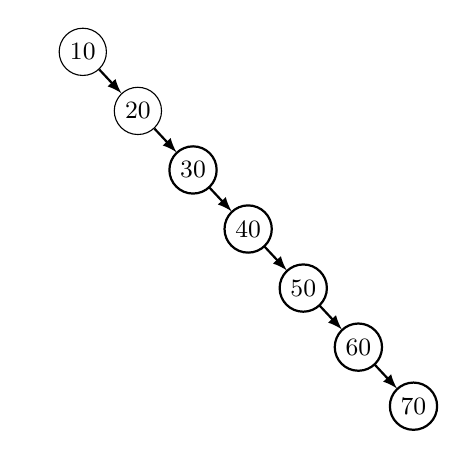
\begin{tikzpicture}[
    level distance=0.75cm,
    sibling distance=1.4cm,
    every node/.style={draw, circle, inner sep=2pt, font=\small, minimum size=6mm},
    edge from parent/.style={draw, -latex, thick}
]
\node {10}
    child { edge from parent[draw=none] }
    child { node {20}
        child { edge from parent[draw=none] }
        child { node {30}
            child { edge from parent[draw=none] }
            child { node {40}
                child { edge from parent[draw=none] }
                child { node {50}
                    child { edge from parent[draw=none] }
                    child { node {60}
                        child { edge from parent[draw=none] }
                        child { node {70} }
                    }
                }
            }
        }
    };
\end{tikzpicture}}

\vspace{0.4cm}
\textbf{Best case (balanced BST)}

\vspace{0.2cm}
\scalebox{1}{
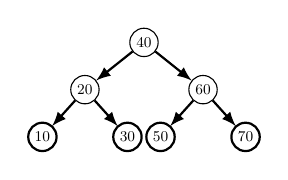
\begin{tikzpicture}[
    level 1/.style={sibling distance=2.5cm},
    level 2/.style={sibling distance=1.8cm},
    level 3/.style={sibling distance=1cm},
    level distance=1cm,
    every node/.style={draw, circle, inner sep=2pt, font=\small, minimum size=6mm},
    edge from parent/.style={draw, -latex, thick},
    scale=0.6,
    transform shape
]
\node {40}
    child { node {20}
        child { node {10} }
        child { node {30} }
    }
    child { node {60}
        child { node {50} }
        child { node {70} }
    };
\end{tikzpicture}}

\end{column}

\end{columns}
\end{frame}

\begin{frame}
\frametitle{2-3 tree}
\begin{itemize}
	\item Tree containing either 2-nodes (2 children) or 3-nodes (3 children).
	\item The 2-nodes work like search trees. The 3-nodes have two values. To the left smaller than the first, in the middle between the first and the second value, to the right larger than the second value.
	\item 2-3 trees are always complete and therefore balanced.
	\item The addition rules are complex to list, BUT intuitive. We go down to where the value should be placed, we add it to the node. If the node becomes a 4-node (three values) we must divide it by moving a value up to the parent node.
\end{itemize}
Everything is in $\mathcal{O}(\log n)$ as a result.
\end{frame}


\begin{frame}[t, fragile] % [t] keeps content at the top
\frametitle{Left-Leaning Red-Black-Trees (LL-RBT) and 2-3 Tree Equivalence}
\begin{columns}[T] 
    
    % Left Column: Text
    \begin{column}{0.55\textwidth}
        \begin{itemize}
            \item \textbf{Search Structure:} A LL-RBT is a BST where red links are only on the left.
            \item \textbf{One-to-One Correspondence:}
            \begin{itemize}
                \item 2-nodes $\rightarrow$ standard black node.
                \item 3-nodes $\rightarrow$ two nodes connected by a \textcolor{red}{red} link.
            \end{itemize}
            \item \textbf{Black Balance:} Every path from root to null link has the same number of black links (perfect black balance).
            \item \textbf{Height:} Guaranteed $O(\log N)$ height; no more than $2 \times \text{height of 2-3 tree}$.
            \item \faExclamationTriangle\ \textbf{Note:} Some textbooks allow right-leaning red links (standard RBT), which are more complex (implementation) to balance.
        \end{itemize}
    \end{column}

    % Right Column: Image
    \begin{column}{0.45\textwidth}
        \begin{figure}
            \centering
            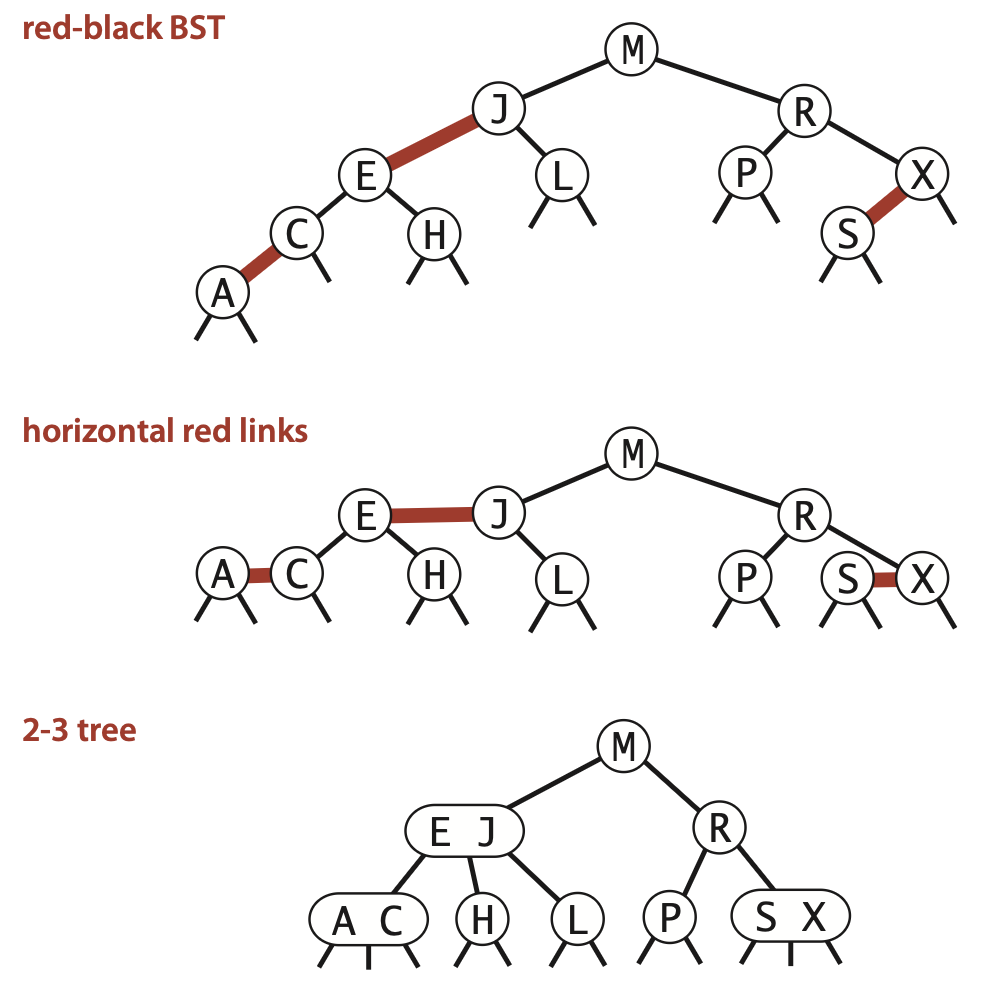
\includegraphics[width=\linewidth]{figures/2-3.png}
        \end{figure}
    \end{column}
    
\end{columns}

\end{frame}




\begin{frame}[fragile]
\frametitle{Hash tables (Separate Chaining)}

\begin{columns}[T]
    % --- Column 1: Theory ---
    \begin{column}{0.45\textwidth}
        \begin{itemize}
            \item \textbf{Principle:} Hash the object key to find an index. Put the (key, value) pair into a bucket at that index.
            \item \textbf{Separate Chaining:} Each bucket `table[i]` points to a linked list of key-value pairs that hashed to the same index `i`.
            \item \textbf{Performance depends on:}
            \begin{itemize}
                \item Quality of hash function.
                \item Load factor ($N/M$).
            \end{itemize}
        \end{itemize}
        \vspace{1em}
        If load factor is kept low (by resizing), operations are $\mathcal{O}(1)$ \textbf{amortized}.
    \end{column}

    % --- Column 2: Pseudocode ---
    \begin{column}{0.52\textwidth}
    \begin{lstlisting}[basicstyle=\tiny\ttfamily, frame=single]
// M = current table size
// N = number of items stored
function insert(key, val)
    // 1. Resize if load factor is too high
    // (e.g., average chain length >= 1)
    if N >= M then
        resize(2 * M) // Rehashes everything

    // 2. Compute index
    i = hash(key) % M

    // 3. Search chain for existing key to update
    for node = table[i]; node != null; node = node.next
        if node.key == key
            node.val = val // Update found
            return

    // 4. Key not found, prepend new node to chain
    oldHead = table[i]
    table[i] = new Node(key, val, next=oldHead)
    N = N + 1
    \end{lstlisting}
    \end{column}
\end{columns}
\end{frame}


\begin{frame}[fragile]
\frametitle{Hash tables (Separate Chaining)}

\begin{columns}[T]
    % --- Column 1: Theory ---
    \begin{column}{0.42\textwidth}
        \begin{itemize}
            \item \textbf{Principle:} Map keys to indices via hashing. Store pairs in "buckets."
            \item \textbf{Separate Chaining:} Buckets are linked lists handling collisions.
            \item \textbf{Dynamic Resizing:} 
            \begin{itemize}
                \item When $N/M$ gets too high, we increase $M$.
                \item \textbf{Rehashing:} Every item must be re-processed because indices change ($hash \pmod M$).
            \end{itemize}
        \end{itemize}
        \vspace{1em}
        Operations are $\mathcal{O}(1)$ \textbf{amortized}.
    \end{column}

    % --- Column 2: Pseudocode ---
    \begin{column}{0.55\textwidth}
    \begin{lstlisting}[basicstyle=\tiny\ttfamily, frame=single]
function insert(key, val)
    if N >= M then resize(2 * M)
    i = hash(key) % M
    for node = table[i]; node != null; node = node.next
        if node.key == key
            node.val = val; return
            
    table[i] = new Node(key, val, next=table[i])
    N = N + 1

function resize(newM)
    newTable = new Array[newM]
    for i = 0 to M - 1
        for node = table[i]; node != null; node = node.next
            // Recompute index for new table size
            newIdx = hash(node.key) % newM
            // Prepend to new chain
            newTable[newIdx] = new Node(node.key, 
                               node.val, next=newTable[newIdx])
    table = newTable
    M = newM
    \end{lstlisting}
    \end{column}
\end{columns}
\end{frame}

\begin{frame}[fragile]
\frametitle{Hash tables - Linear Probing}

\begin{columns}[T]
    % --- Column 1: Theory ---
    \begin{column}{0.45\textwidth}
        \begin{itemize}
            \item \textbf{Collision Resolution:} If `table[i]` is occupied, try `i+1`, `i+2`, etc. (wrapping around).
            \item \textbf{Insertion:} Find the first empty slot in the sequence.
            \item \textbf{Search:} Follow the probe sequence until the key is found or an empty slot is reached.
            \item \textbf{The Deletion Problem:}
            \begin{itemize}
                \item You cannot simply set a slot to `null`.
                \item This would break the probe chain for items inserted *after* it in the same cluster.
                \item \textbf{Fix:} Use "tombstones" or re-insert subsequent items in the cluster.
            \end{itemize}
        \end{itemize}
    \end{column}

    % --- Column 2: Pseudocode ---
    \begin{column}{0.52\textwidth}
    \begin{lstlisting}[basicstyle=\tiny\ttfamily, frame=single]
// M = table size, keys[] and vals[] arrays

function put(key, val)
    i = hash(key)
    // Stop at null (empty) or existing key
    while keys[i] != null
        if keys[i] == key
            vals[i] = val // Update
            return
        i = (i + 1) % M // Wrap around
    
    // Found empty slot
    keys[i] = key
    vals[i] = val
    N = N + 1

function get(key)
    i = hash(key)
    while keys[i] != null
        if keys[i] == key
            return vals[i]
        i = (i + 1) % M
    return null // Not found
    \end{lstlisting}
    \end{column}
\end{columns}

\end{frame}


\begin{frame}[fragile]
\frametitle{LRU Cache Implementation}

\begin{columns}[T]
    % --- Column 1: The Concept ---
    \begin{column}{0.45\textwidth}
        \textbf{Goal:} $\mathcal{O}(1)$ for both `get` and `put`.
        
        \vspace{0.5em}
        We combine two data structures:
        \begin{itemize}
            \item \textbf{Doubly Linked List (DLL):}
            \begin{itemize}
                \item Maintains usage order.
                \item \textbf{Head:} Most Recently Used (MRU).
                \item \textbf{Tail:} Least Recently Used (LRU) - candidate for eviction.
            \end{itemize}
            \item \textbf{Hash Map:}
            \begin{itemize}
                \item Maps `Key` $\to$ the specific `DLL Node`.
                \item Allows jumping directly to a node in the middle of the list without traversal.
            \end{itemize}
        \end{itemize}
    \end{column}

    % --- Column 2: Pseudocode ---
    \begin{column}{0.52\textwidth}
    \begin{lstlisting}[basicstyle=\tiny\ttfamily, frame=single]
class Node { key, val, prev, next }
Map<Key, Node> map
Node head, tail // Dummy sentinels

function get(key)
    if key not in map then return null
    node = map[key]
    // Move to front (MRU position)
    removeNode(node)
    addToHead(node)
    return node.val

function put(key, val)
    if key in map
        node = map[key]
        node.val = val
        // Update usage: move to front
        removeNode(node)
        addToHead(node)
    else
        newNode = new Node(key, val)
        map[key] = newNode
        addToHead(newNode)
        if map.size() > capacity
            // Evict LRU (item before tail)
            lru = tail.prev
            removeNode(lru)
            map.remove(lru.key)
\end{lstlisting}
    \end{column}
\end{columns}

\end{frame}




\begin{frame}[fragile]
\frametitle{Rabin-Karp Algorithm}

\begin{columns}[T]
    % --- Column 1: Theory & Math ---
    \begin{column}{0.48\textwidth}
        \textbf{Goal:} efficient search for fixed-length ($M$) patterns in a text.
        \begin{itemize}
            \item \textbf{Preprocessing:} Hash all patterns and store in a \texttt{Map<Long, String>}.
            \item \textbf{Rolling Hash:} Update the hash in $\mathcal{O}(1)$ as the window slides.
            \item \textbf{Verification:} If hash matches, compare actual characters to rule out collisions.
        \end{itemize}
        
        \vspace{0.5em}
        \textbf{The Math (Polynomial Hash):}
        $$ H_i = \sum_{j=0}^{M-1} x_{i+j} R^{M-1-j} $$
        
        \textbf{Rolling Update:} To move window $i \to i+1$:
        \begin{enumerate}
            \item Remove leading char $x_i$ ($x_i R^{M-1}$).
            \item Shift left (multiply by $R$).
            \item Add new trailing char $x_{i+M}$.
        \end{enumerate}
        $$ H_{i+1} = (H_i - x_i R^{M-1}) \cdot R + x_{i+M} $$
    \end{column}

    % --- Column 2: Pseudocode ---
    \begin{column}{0.48\textwidth}
    \begin{lstlisting}[basicstyle=\tiny\ttfamily, frame=single]
function rabinKarp(txt, patterns, M)
    map = new HashMap()
    RM = pow(R, M-1) // Precompute multiplier
    
    // 1. Preprocess patterns
    for p in patterns
        map.put(hash(p), p)

    // 2. Compute hash of first window
    h = hash(txt[0...M-1])

    // 3. Roll through text
    for i from 0 to N - M
        // Check for match
        if map.contains(h)
            // Handle Collisions
            if txt[i...i+M-1] == map.get(h)
                return i // Match found

        // Roll hash (avoid loop!)
        if i < N - M
            // Remove leading, shift, add trailing
            h = (h - txt[i] * RM) * R + txt[i+M]
            // (Apply modulo Q here in practice)
            
    return -1
    \end{lstlisting}
    \end{column}
\end{columns}

\end{frame}


\begin{frame}[fragile]
\frametitle{Huffman compression}
\begin{columns}[T]
    % --- Column 1: Explanation ---
    \begin{column}{0.4\textwidth}
        \begin{itemize}
            \item Start with a set of trees, each corresponding to a character's frequency.
            \item Use a Min-Priority Queue to store these trees.
            \item Repeat until only one tree remains:
            \item Extract the two smallest frequency trees ($x$ and $y$).
            \item Merge them into a new tree with frequency $x.freq + y.freq$.
            \item Insert the new tree back into the PQ.
        \end{itemize}
        \vspace{1em}
        $\mathcal{O}(n \log n)$ where $n$ is the number of characters.
    \end{column}

    % --- Column 2: Pseudocode ---
    \begin{column}{0.58\textwidth}
    \begin{lstlisting}[basicstyle=\tiny\ttfamily, frame=single]
function buildHuffmanTree(frequencies)
    PQ = new MinPriorityQueue()
    
    // Create leaf node for each char
    for char, count in frequencies
        node = new Node(char, count)
        PQ.insert(node)

    // Merge nodes until one remains
    while PQ.size() > 1
        x = PQ.extractMin()
        y = PQ.extractMin()
        
        sum = x.freq + y.freq
        // Create new internal node
        z = new Node(sum, left=x, right=y)
   
        PQ.insert(z)

    return PQ.extractMin() // The root
    \end{lstlisting}
    \end{column}
\end{columns}
\end{frame}

\begin{frame}[fragile]
\frametitle{Union-Find (Weighted Quick-Union)}

\begin{columns}[T]
    % --- Column 1: Concepts & Strategy ---
    \begin{column}{0.48\textwidth}
        \textbf{Concept:} Maintain disjoint sets as trees using an array `parent`.
        \begin{itemize}
            \item \textbf{Representative:} The root of the tree (`parent[i] == i`).
            \item \textbf{Weighted Union:} Always link the \textit{smaller} tree to the \textit{larger} tree (maintains balance).
            \item \textbf{Path Compression:} During `find`, make nodes point directly to the root.
        \end{itemize}
        
        \vspace{1em}
        \textbf{Complexity:} \\
        $\mathcal{O}(\log n)$ with weighted union. \\
        $\mathcal{O}(\alpha(n))$ with weighted union + path compression.
    \end{column}

    % --- Column 2: Implementation ---
    \begin{column}{0.48\textwidth}
    \begin{lstlisting}[basicstyle=\tiny\ttfamily, frame=single]
int[] parent, size

function find(i)
    if parent[i] == i then return i
    
    // Path Compression:
    // Point i directly to the root
    parent[i] = find(parent[i])
    
    return parent[i]

function union(p, q)
    rootP = find(p)
    rootQ = find(q)
    if rootP == rootQ return

    // Weighted: small to large
    if size[rootP] < size[rootQ]
        parent[rootP] = rootQ
        size[rootQ] += size[rootP]
    else
        parent[rootQ] = rootP
        size[rootP] += size[rootQ]
    \end{lstlisting}
    \end{column}
\end{columns}

\end{frame}

\begin{frame}
\frametitle{A quick reminder about graphs}
\begin{itemize}
	\item Graph: set of nodes and edges connecting these nodes. ($G=<V,E>$)
	\item \textit{Weighted} graph: the edges have an associated weight. Mathematically, usually, we define this via a function $f: E \rightarrow \mathbb{R}$ which gives a weight when given an edge.
	\item \textit{Simple} graph: there is, between any pair of nodes, at most one edge. This implies that $E \leq \frac{V\cdot(V-1)}{2} \in \mathcal{O}(V^2)$ and therefore that $\mathcal{O}(\log E) \subseteq \mathcal{O}(\log V^2) = \mathcal{O}(2 \log V) = \mathcal{O}(\log V)$.
	\item \textit{Directed} graph: the edges have a direction. Generally, we then call these edges \textit{arcs}.
	\item Degree of a node: number of edges touching a node.
	\item In-degree (resp. out-degree): number of arcs of which the node is the destination (resp. origin).
	\item Sum of the degrees of the nodes = $2E$
	\item \textit{Acyclic} graph: without a cycle (directed or not, depending on the case).
\end{itemize}
\end{frame}

\begin{frame}[t, fragile]
\frametitle{Graph ADT: Adjacency Matrix vs. List}

\begin{columns}[T]
    % --- Left Column: Implementations ---
    \begin{column}{0.5\textwidth}
        \textbf{1. Adjacency Matrix}
        \begin{itemize}
            \item A 2D array \texttt{adj[V][V]} where \texttt{adj[u][v] == 1} if edge $(u,v)$ exists.
        \end{itemize}
        \begin{lstlisting}[language=Java, basicstyle=\tiny\ttfamily, frame=leftline]
boolean[][] adj = new boolean[V][V];
void addEdge(u, v) { adj[u][v] = true; }
        \end{lstlisting}

        \vspace{0.2cm}
        \textbf{2. Adjacency List}
        \begin{itemize}
            \item An array of $V$ lists; \texttt{adj[u]} contains all neighbors of $u$.
        \end{itemize}
        \begin{lstlisting}[language=Java, basicstyle=\tiny\ttfamily, frame=leftline]
List<Integer>[] adj = new List[V];
void addEdge(u, v) { adj[u].add(v); }
        \end{lstlisting}
    \end{column}

    % --- Right Column: Comparison ---
    \begin{column}{0.5\textwidth}
        \textbf{Pros, Cons \& Complexity}
        
        \vspace{0.1cm}
        \scriptsize
        \renewcommand{\arraystretch}{1.3}
        \begin{tabular}{|l|c|c|}
        \hline
        \textbf{Operation} & \textbf{Matrix} & \textbf{List} \\ \hline
        \textbf{Space} & $O(V^2)$ & $O(V + E)$ \\ \hline
        \textbf{Add Edge} & $O(1)$ & $O(1)$ \\ \hline
        \textbf{Check Edge} & $O(1)$ & $O(degree(u))$ \\ \hline
        \textbf{Iterate neighbors} & $O(V)$ & $O(degree(u))$ \\ \hline
        \end{tabular}

        \vspace{0.3cm}
        \normalsize \textbf{When to use?}
        \begin{itemize}
            \item \textbf{Matrix:} \textbf{Dense} graphs ($E \approx V^2$) or when you need constant-time edge lookups.
            \item \textbf{List:} \textbf{Sparse} graphs (most real-world cases). Memory efficient and faster for traversing neighbors.
        \end{itemize}
    \end{column}
\end{columns}

\end{frame}



\begin{frame}[t, fragile]
\frametitle{Breadth-First Search (BFS)}

\begin{columns}[T]
    % --- Left Column: Logic & Properties ---
    \begin{column}{0.48\textwidth}
        \textbf{Concepts}
        \begin{itemize}
            \item \textbf{Layer-by-layer:} Visits all nodes at distance $d$ before moving to $d+1$.
            \item \textbf{What it computes:}
            \begin{itemize}
            	\item In unweighted graphs, BFS finds the minimum number of hops from source $s$ to any reachable $v$.
                \item \texttt{dist[v]}: Shortest path length of $s \to v$.
                \item \texttt{prev[v]}: The node that "discovered" $v$.
            \end{itemize}
            \item \textbf{Path Reconstruction:} Following \texttt{prev[]} pointers backwards from $v$ yields the shortest path to $s$.
        \end{itemize}
        \textbf{Complexity:} $\mathcal{O}(V+E)$
    \end{column}

    % --- Right Column: Pseudocode ---
    \begin{column}{0.52\textwidth}
\begin{lstlisting}[language=Java, basicstyle=\tiny\ttfamily, frame=single, title=BFS(Graph G\, Source s)]
Queue q = new Queue();
boolean[] visited = new boolean[G.V()];
int[] dist = new int[G.V()];
int[] prev = new int[G.V()]; // Path tree

visited[s] = true;
q.enqueue(s);

while (!q.isEmpty()) {
    int u = q.dequeue();
    for (int v : G.adj(u)) {
        if (!visited[v]) {
            visited[v] = true;
            dist[v] = dist[u] + 1;
            prev[v] = u; // Discovery link
            q.enqueue(v);
        }
    }
}
\end{lstlisting}
    \end{column}
\end{columns}
\end{frame}

\begin{frame}[t, fragile]
\frametitle{Depth-First Search (DFS)}

\begin{columns}[T]
    % --- Left Column: Logic & Properties ---
    \begin{column}{0.48\textwidth}
        \begin{itemize}
            \item \textbf{Intuition} Explores as far as possible along each branch before backtracking.
            \item \textbf{What it computes:}
            \begin{itemize}
            	\item Finds \textit{a} path from $s$ to $v$, but it is \textbf{not necessarily the shortest}.
                \item \texttt{visited[v]}: Keeps track of nodes already explored.
                \item \texttt{prev[v]}: Encodes the path tree (the "parent" node in the recursion).
            \end{itemize}
            \item \textbf{Possible implems:} Uses the call stack (Recursion) or an explicit \textbf{Stack} (LIFO).
            \item \textbf{Path Reconstruction:} Following \texttt{prev[]} pointers backwards from $v$ yields a path to $s$ (not necessarily the shortest).
            \item \textbf{Complexity:} $\mathcal{O}(V+E)$.
           \item Can be used for directed or undirected graph.
        \end{itemize}
        
    \end{column}

    % --- Right Column: Pseudocode ---
    \begin{column}{0.52\textwidth}
\begin{lstlisting}[language=Java, basicstyle=\tiny\ttfamily, frame=single, title=DFS(Graph G\, Source s)]
boolean[] visited = new boolean[G.V()];
int[] prev = new int[G.V()];
search(G, s) // Initial call

void search(Graph G, int u) {
    visited[u] = true;
    for (int v : G.adj(u)) {
        if (!visited[v]) {
            prev[v] = u; // Record discovery
            search(G, v); // Recursive dive
        }
    }
}
\end{lstlisting}
    \end{column}
\end{columns}
\end{frame}



\begin{frame}[t, fragile]
\frametitle{Depth-First Search (DFS)}

\begin{columns}[T]
    % --- Left Column: Logic & Properties ---
    \begin{column}{0.48\textwidth}
        \begin{itemize}
            \item \textbf{Deep Dive:} Explores as far as possible along each branch before backtracking.
            \item \textbf{Path Finding:} Finds \textit{a} path from $s$ to $v$, but it is \textbf{not necessarily the shortest}.
            \item \textbf{Discovery State:}
            \begin{itemize}
                \item \texttt{visited[v]}: Keeps track of nodes already explored.
                \item \texttt{prev[v]}: Encodes the path tree (the "parent" node in the recursion).
            \end{itemize}
            \item \textbf{Mechanism:} Uses the call stack (Recursion) or an explicit \textbf{Stack} (LIFO).
            \item \textbf{Complexity:} $\mathcal{O}(V+E)$.
            \item Can be used for directed or undirected graph.
        \end{itemize}
    \end{column}

    % --- Right Column: Pseudocode ---
    \begin{column}{0.52\textwidth}
\begin{lstlisting}[language=Java, basicstyle=\tiny\ttfamily, frame=single, title=DFS(Graph G\, Source s)]
boolean[] visited = new boolean[G.V()];
int[] prev = new int[G.V()];

void search(Graph G, int u) {
    visited[u] = true;
    for (int v : G.adj(u)) {
        if (!visited[v]) {
            prev[v] = u; // Record discovery
            search(G, v); // Recursive dive
        }
    }
}

// Initial call: search(G, s)
\end{lstlisting}
    \end{column}
\end{columns}
\end{frame}



\begin{frame}[t, fragile]
\frametitle{DFS Applications in $\mathcal{O}(V+E)$}
\begin{columns}[T]
    % --- Left Column: Cycle Detection ---
    \begin{column}{0.5\textwidth}
        \textbf{1. (Directed) cycle detection in a (directed) graph}\\
        A cycle exists if we visit an \textbf{Open} node:
        \begin{itemize}
                    \item \textbf{0 (Unseen):} Default.
                    \item \textbf{1 (Open):} Node is on the \textbf{current} recursion stack.
                    \item \textbf{2 (Closed):} Node \& all descendants visited.
        \end{itemize}
        \begin{lstlisting}[basicstyle=\tiny\ttfamily, frame=single]
int[] state; // 0: UNSEEN, 1: OPEN, 2: CLOSED
public boolean hasCycle() {
    state = new int[V]; 
    for (int i = 0; i < V; i++) {
        if (state[i] == 0) {
            if (hasCycle(i)) return true;
        }
    }
    return false;
}
bool hasCycle(int u) {
    state[u] = 1; // Mark OPEN (on stack)
    for (int v : adj[u]) {
        if (state[v] == 0 && hasCycle(v)) return true;
        if (state[v] == 1) return true; // Cycle!
    }
    state[u] = 2; // Mark CLOSED (backtrack)
    return false;
}
        \end{lstlisting}
    \end{column}

    % --- Right Column: Bipartite Testing ---
    \begin{column}{0.5\textwidth}
        \textbf{2. Test if an undirected graph is bipartite}
        \begin{itemize}
            \item \textbf{Logic:} Assign alternate colors (0 and 1).
            \item \textbf{Conflict:} A neighbor already has the \textbf{same} color as current node $\rightarrow$ not bipartite.
        \end{itemize}
        \begin{lstlisting}[basicstyle=\tiny\ttfamily, frame=single]
int[] color; // -1: NONE, 0: RED, 1: BLUE
public boolean isBipartite() {
    color = new int[V];
    Arrays.fill(color, -1);
    for (int i = 0; i < V; i++) {
        if (color[i] == -1) { 
            if (!isBipartite(i, 0)) return false;
        }
    }
    return true; // All components successfully 2-colored
}
bool isBipartite(int u, int c) {
    color[u] = c; // Color this node
    for (int v : adj[u]) {
        if (color[v] == -1) { // Not visited
            if (!isBipartite(v, 1-c)) return false;
        } else if (color[v] == c) {
            return false; // Conflict found!
        }
    }
    return true;
}
        \end{lstlisting}
    \end{column}
\end{columns}
\end{frame}

\begin{frame}[t, fragile]
\frametitle{Topological Sort}

\begin{columns}[T]
    % --- Left Column: Concept ---
    \begin{column}{0.45\textwidth}
        \textbf{Objective}
        \begin{itemize}
            \item For a \textbf{DAG}, find an ordering where for every edge $(u, v)$, $u$ comes before $v$.
            \item \textbf{Intuition:} "Unlock" nodes only after all their prerequisites are met.
        \end{itemize}
        \vspace{0.3cm}
        \textbf{In-degree Check}
        \begin{itemize}
            \item If at the end the order contains fewer than $V$ nodes, the graph has a \textbf{cycle}.
        \end{itemize}
        \textbf{Complexity:} $\mathcal{O}(V+E)$
    \end{column}

    % --- Right Column: Pseudocode ---
    \begin{column}{0.55\textwidth}
\begin{lstlisting}[language=Java, basicstyle=\tiny\ttfamily, frame=single]
// 1. Calculate in-degree for all nodes
int[] inDegree = new int[V];
for (int u = 0; u < V; u++)
    for (int v : adj[u]) inDegree[v]++;

// 2. Queue all nodes with no dependencies
Queue q = new Queue();
for (int i = 0; i < V; i++)
    if (inDegree[i] == 0) q.enqueue(i);

// 3. Process the queue
List order = new ArrayList();
while (!q.isEmpty()) {
    int u = q.dequeue();
    order.add(u);
    for (int v : adj[u]) {
        inDegree[v]--; // "Remove" edge (u, v)
        if (inDegree[v] == 0) q.enqueue(v);
    }
}
\end{lstlisting}
    \end{column}
\end{columns}
\end{frame}



\begin{frame}[t, fragile]
\frametitle{Minimum Spanning Tree Algorithms: Prim vs. Kruskal}
\begin{block}{Definitions}
    \begin{itemize}
        \item \textbf{Spanning Tree:} Connected acyclic graph ($n$ nodes $\Rightarrow n-1$ edges).
        \item \textbf{Minimum Weight:} No spanning tree exists with a smaller total edge sum.
    \end{itemize}
\end{block}
\begin{columns}[T]
    % --- Left Column: Prim ---
    \begin{column}{0.5\textwidth}
        \textbf{Prim's (Vertex-Centric)}
        \textit{"Grow a single tree"}
        \begin{itemize}
            \item Start from an arbitrary node.
            \item Always pick the cheapest edge connecting the tree to a \textit{new} node.
        \end{itemize}
        \begin{lstlisting}[basicstyle=\tiny\ttfamily, frame=single, title=Prim(G)]
PriorityQueue pq;
pq.addEdges(startNode);
while (!pq.isEmpty()) {
    Edge e = pq.poll();
    if (e.to is visited) continue;
    
    add e to MST;
    visit(e.to);
    pq.addEdges(e.to neighbors);
}
        \end{lstlisting}
    \end{column}

    % --- Right Column: Kruskal ---
    \begin{column}{0.5\textwidth}
        \textbf{Kruskal's (Edge-Centric)}
        \textit{"Merge separate forests"}
        \begin{itemize}
            \item Sort all edges by weight.
            \item Pick the cheapest edge that doesn't create a cycle (using \textbf{Union-Find}).
        \end{itemize}
        \begin{lstlisting}[basicstyle=\tiny\ttfamily, frame=single, title=Kruskal(G)]
sort edges by weight;
UnionFind uf = new UF(V);
for (Edge e : edges) {
    if (!uf.connected(e.u, e.v)) {
        uf.union(e.u, e.v);
        add e to MST;
    }
    if (MST.size == V-1) break;
}
        \end{lstlisting}
    \end{column}
\end{columns}

\vspace{0.2cm}
\centering
\textbf{Complexity for both:} $\mathcal{O}(E \log V)$ or $\mathcal{O}(E \log E)$
\end{frame}

\begin{frame}[t, fragile]
\frametitle{Shortest Path: Dijkstra's Algorithm (Lazy Implementation: no priority update)}
\begin{columns}[T]
    % --- Left Column: Concept ---
    \begin{column}{0.45\textwidth}
        \textbf{Concepts}
        \begin{itemize}
            \item \textbf{Greedy Choice:} Always expand the node with the smallest current distance.
            \item \textbf{Relaxation:} If \texttt{dist[u] + w < dist[v]}, we found a better path.
            \item \textbf{Lazy Update:} Instead of updating a value in the PQ, we insert a \textit{new} entry because the \textit{PriorityQueue} of Java does not support priority update.
            \item \textbf{Condition:} We only process a node if the distance popped matches the \texttt{dist[]} array.
            \item \faExclamationTriangle\ Dijstra does not work if negative edge weights.
        \end{itemize}
        \textbf{Complexity:} $\mathcal{O}(E \log V)$
    \end{column}

    % --- Right Column: Pseudocode ---
    \begin{column}{0.55\textwidth}
\begin{lstlisting}[language=Java, basicstyle=\tiny\ttfamily, frame=single, title=Dijkstra(Graph G\, s)]
dist[] = new int[V]; // Init with infinity
prev[] = new int[V]; 
PriorityQueue<Node> pq = new PriorityQueue<>();

dist[s] = 0;
pq.add(new Node(s, 0));

while (!pq.isEmpty()) {
    Node current = pq.poll();
    int u = current.id;
    int d = current.distance;

    // Skip if already found a shorter path to u
    if (d > dist[u]) continue;

    for (Edge e : G.adj(u)) {
        int v = e.to;
        if (dist[u] + e.weight < dist[v]) {
            dist[v] = dist[u] + e.weight;
            prev[v] = u;
            pq.add(new Node(v, dist[v]));
        }
    }
}
\end{lstlisting}
    \end{column}
\end{columns}
\end{frame}

\begin{frame}[t, fragile]
\frametitle{Bellman-Ford Algorithm}

\begin{columns}[T]
    % --- Left Column: Concept ---
    \begin{column}{0.48\textwidth}
        \begin{itemize}
            \item Computes shortest paths with at most 1 edge, then $2$, $\ldots$ , up to $V-1$.
            \item Unlike Dijkstra, it handles negative edge weights correctly.
            \item If a distance can still be reduced in the $V$-th iteration, a \textbf{negative cycle} exists.
        \end{itemize}
        \vspace{0.2cm}
        \textbf{Complexity:} $\mathcal{O}(V \times E)$.
    \end{column}

    % --- Right Column: Java-like Implementation ---
    \begin{column}{0.52\textwidth}
\begin{lstlisting}[language=Java, basicstyle=\tiny\ttfamily, frame=single, title=BellmanFord(List<Edge> edges\, int s)]
double[] dist = new double[V];
Arrays.fill(dist, Double.POSITIVE_INFINITY);
dist[s] = 0.0;

// Relax all edges V-1 times
for (int i = 1; i < V; i++) {
    for (Edge e : edges) {
        if (dist[e.u] + e.weight < dist[e.v]) {
            dist[e.v] = dist[e.u] + e.weight;
        }
    }
}

// Check for negative cycles
for (Edge e : edges) {
    if (dist[e.u] + e.weight < dist[e.v]) {
        throw new RuntimeException("Negative cycle!");
    }
}

return dist;
\end{lstlisting}
    \end{column}
\end{columns}
\end{frame}

\begin{frame}[fragile]
\frametitle{Floyd-Warshall}
\begin{itemize}
	\item Calculation of all the shortest path distances between all pairs of nodes, in a \textbf{weighted} directed graph of $V$ nodes. You get the distances at the end, but not the paths.
	\item Proof by induction on $k$: $d[i][j]$ is the distance of the shortest path using only detours in $\{1..k-1\}$.
\end{itemize}

    \begin{lstlisting}[basicstyle=\tiny\ttfamily, frame=single]
function Floyd_Warshall(G)
    d[i][j] = (i,j) in E ? weight(i,j), (+inf) otherwise
    for k from 1 to V-1 do
        for i from 1 to V-1 do
            for j from 1 to V-1 do
                d[i][j] = min(d[i][j],d[i][k]+d[k][j])
    return d
\end{lstlisting}
$\mathcal{O}(V^3)$
\end{frame}



\begin{frame}[fragile]
\frametitle{Longest path}
\begin{itemize}
	\item It is conjectured that there is no polynomial time algorithm to find the longest path in an arbitrary graph (NP-Complete problem).
	\item If the graph is a DAG (directed acyclic graph) then there is a polynomial algorithm: take the opposite of the edge weights, and use Bellman-Ford.
	\item This works because there will be negative weights, but no negative cycles since the graph is acyclic.
\end{itemize}
\end{frame}

\section{Tips \& tricks}

\begin{frame}[fragile]
\frametitle{Iterating over collections}
{\color{red} I NEVER want to see this:}
\begin{lstlisting}
List<String> x = ...;
for(int i = 0; i < x.size(); i++) {
	String elem = x.get(i);
	//...
}
\end{lstlisting}
{\color{red} This is $\mathcal{O}(n^2)$!}

{\color{blue} Please use foreach:}
\begin{lstlisting}
for(String elem: x) {
	//...
}
\end{lstlisting}

{\color{blue} Or an iterator:}
\begin{lstlisting}
Iterator<String> itr = x.iterator();
while(itr.hasNext()) {
	String elem = itr.next();
	//...
}
\end{lstlisting}
\end{frame}

\begin{frame}[fragile]
\frametitle{Iterating over collections (2)}
For dictionaries (\texttt{HashMap}, \texttt{TreeMap}), three reasonable possibilities:
\begin{lstlisting}
HashMap<X, Y> hashmap = ...;
for(Map.Entry<X, Y> pair: hashmap.entrySet()) {
	X key = pair.getKey();
	Y value = pair.getValue();
	// ...
}
\end{lstlisting}

\begin{lstlisting}
for(X key: hashmap.keySet()) {
	Y value = hashmap.get(key);
	// ...
}
\end{lstlisting}

Or with an iterator (on \texttt{hashmap.entrySet().iterator()} or \texttt{hashmap.keySet().iterator()}).

If you use a TreeMap, it's given in sorted order! Be careful that it's always $\mathcal{O}(n)$ except in the second case with the TreeMap, where it's $\mathcal{O}(n \log n)$.
\end{frame}

\end{document}
